%%%%%%%%%%%%%%%%%%%%%%%%%%%%%%%%%%%%%%%%%%%%%%%%%%%%%%%%%%%%%%%%%%%%%%%%%%%%%%%%%%%%%%%
%%%%%%%%%%%%%%%%%%%%%%%%%%%%%%%%%%%%%%%%%%%%%%%%%%%%%%%%%%%%%%%%%%%%%%%%%%%%%%%%%%%%%%%
% 
% This top part of the document is called the 'preamble'.  Modify it with caution!
%
% The real document starts below where it says 'The main document starts here'.


\documentclass[12pt]{article}

\usepackage{amssymb,amsmath,amsthm}
\usepackage[top=1in, bottom=1in, left=1.25in, right=1.25in]{geometry}
\usepackage{fancyhdr}
\usepackage{listings}
\usepackage{enumerate}
\usepackage{hieroglf}
\usepackage{oands}
\usepackage{arevmath}
\usepackage{relsize}
\usepackage{times,txfonts}
\usepackage{graphicx}
\usepackage{float}

\newtheoremstyle{homework}% name of the style to be used
  {18pt}% measure of space to leave above the theorem. E.g.: 3pt
  {12pt}% measure of space to leave below the theorem. E.g.: 3pt
  {}% name of font to use in the body of the theorem
  {}% measure of space to indent
  {\bfseries}% name of head font
  {:}% punctuation between head and body
  {2ex}% space after theorem head; " " = normal interword space
  {}% Manually specify head
\theoremstyle{homework} 

% Set up an Exercise environment and a Solution label.
\newtheorem*{exercisecore}{Exercise \@currentlabel}
\newenvironment{exercise}[1]
{\def\@currentlabel{#1}\exercisecore}
{\endexercisecore}

\newcommand{\localhead}[1]{\par\smallskip\noindent\textbf{#1}\nobreak\\}%
\newcommand\solution{\localhead{Solution:}}

%%%%%%%%%%%%%%%%%%%%%%%%%%%%%%%%%%%%%%%%%%%%%%%%%%%%%%%%%%%%%%%%%%%%%%%%
%
% Stuff for getting the name/document date/title across the header
\makeatletter
\RequirePackage{fancyhdr}
\pagestyle{fancy}
\fancyfoot[C]{\ifnum \value{page} > 1\relax\thepage\fi}
\fancyhead[L]{\ifx\@doclabel\@empty\else\@doclabel\fi}
\fancyhead[C]{\ifx\@docdate\@empty\else\@docdate\fi}
\fancyhead[R]{\ifx\@docauthor\@empty\else\@docauthor\fi}
\headheight 15pt

\def\doclabel#1{\gdef\@doclabel{#1}}
\doclabel{Use {\tt\textbackslash doclabel\{MY LABEL\}}.}
\def\docdate#1{\gdef\@docdate{#1}}
\docdate{Use {\tt\textbackslash docdate\{MY DATE\}}.}
\def\docauthor#1{\gdef\@docauthor{#1}}
\docauthor{Use {\tt\textbackslash docauthor\{MY NAME\}}.}
\makeatother

% Shortcuts for blackboard bold number sets (reals, integers, etc.)
\newcommand{\Reals}{\ensuremath{\mathbb R}}
\newcommand{\Nats}{\ensuremath{\mathbb N}}
\newcommand{\Ints}{\ensuremath{\mathbb Z}}
\newcommand{\Rats}{\ensuremath{\mathbb Q}}
\newcommand{\Cplx}{\ensuremath{\mathbb C}}
%% Some equivalents that some people may prefer.
\let\RR\Reals
\let\NN\Nats
\let\II\Ints
\let\CC\Cplx

%%%%%%%%%%%%%%%%%%%%%%%%%%%%%%%%%%%%%%%%%%%%%%%%%%%%%%%%%%%%%%%%%%%%%%%%%%%%%%%%%%%%%%%
%%%%%%%%%%%%%%%%%%%%%%%%%%%%%%%%%%%%%%%%%%%%%%%%%%%%%%%%%%%%%%%%%%%%%%%%%%%%%%%%%%%%%%%
% 
% The main document start here.

% The following commands set up the material that appears in the header.
\doclabel{Math 316: HW 3}
\docauthor{Stefano Fochesatto}
\docdate{\today}

\begin{document}


\textbf{Section 3.4}
\begin{enumerate}
\setcounter{enumi}{1}
\item  The following solution to the continued mean proportionals problem is often attributed to Plato, although
it could hardly be his in view of his objection to mechanical constructions. Consider two right triangles $ABC$ and 
$BCD$, lying on the same side of he common leg $BC$. Suppose that the hypotenuses $AC$ and $BD$ intersect perpendicularly
at point $P$, and are constructed in such a way that $AP= a$ and $DP = 2a$. Prove that $x = BP$ and $y = CP$ are the required mean proportionals between 
$a$ and $2a$, that is, 
\begin{equation*}
  \frac{a}{x} = \frac{x}{y} = \frac{y}{2a}.
\end{equation*}
\begin{center}
  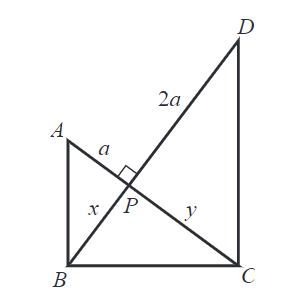
\includegraphics[width = .33\textwidth]{meanprop.png}
\end{center}
\textbf{Answer:} Note that since $ABC$ and $BCD$ are right triangles with the following property, 
\begin{equation*}
  \angle ABC = \angle DCB = 90^{\circ}
\end{equation*}  
Note that these angles sum to $180^{\circ}$ and are the interior angles to segments $AB$ and $DC$. Therefore by Euclid's Parallel postulate 
$AB$||$DC$. With segments $AC$ and $BD$ as transversals we get the following equalities through alternate interior angles.
\begin{equation*}
  \angle BAC = \angle DCA,
\end{equation*}
\begin{equation*}
  \angle ABD = \angle CDB.
\end{equation*}
Therefore we get $\triangle APB \sim \triangle CPD$ by AA similarity. Note that by the construction of point $P$ and vertical angles we know that,
\begin{equation*}
  \angle DPA = \angle BPC = \angle APB = \angle CPD = 90^{\circ}.
\end{equation*}  
Since the angles of  $\triangle BCD$ and $\triangle CPD$ sum $180^{\circ}$
we get the following through algebra, 
\begin{align*}
  \angle CDB + \angle DCP + 90^{\circ} &= \angle CDB + \angle CBD + 90^{\circ},\\
  \angle DCP &= \angle CBD.
\end{align*}
Note that $\angle CBP = \angle CBD = \angle DCP$ and $\angle BPC =\angle CPD$ therefore by AA similarity $\triangle BPC \sim \triangle CPD$. Thus by 
the transitivity of similar triangles we know that $\triangle APB \sim \triangle CPD \sim \triangle BPC$ and the desired proportional relationship,
\begin{equation*}
  \frac{a}{x} = \frac{x}{y} = \frac{y}{2a}
\end{equation*}
is derived from the ratio between the legs of each right triangle. 
\vspace{.5in}



\setcounter{enumi}{3}
\item The Greek mathematician Menaechmus, the tutor of Alexander the Great, obtained a purely theoretical solution to the duplication problem
based on finding the point of intersection of certain conic sections. To duplicate a cube of edge $a$, he constructed two parabolas having a common vertex
and perpendicular axes, so that one parabola had a focal chord of length $a$ and the other a chord of length $2a$. Prove that the abscissa $x$ of the point of 
intersection of the two parabolas satisfies the condition $x^3 = 2a^3$; the sought for $x$, the cube's edge, is thereby obtained. 
\begin{center}
  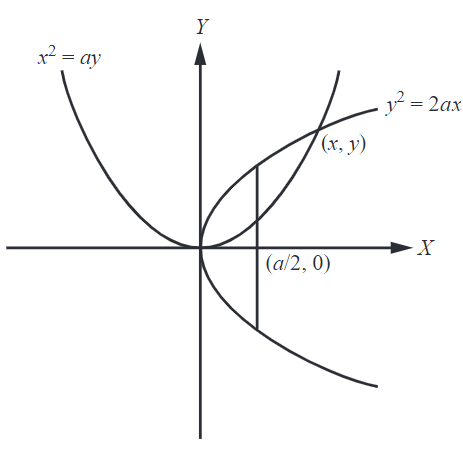
\includegraphics[width = .33\textwidth]{conic.png}
\end{center}
\textbf{Answer:} Using modern methods we can do this by solving both equations for $y$ and then setting them equal to each other. 
\begin{align*}
  x^2 &= ay,\\
  \frac{x^2}{a} &= y.
\end{align*}
\begin{align*} 
  y^2 &= 2ax,\\
  y &= (2ax)^{\frac{1}{2}}.
\end{align*}
Finally we get that,
\begin{align*}
  \frac{x^2}{a} &= (2ax)^{\frac{1}{2}},\\
  \frac{x^4}{a^2} &= 2ax,\\
  x^4 &= 2a^3x,\\
  x^3 &= 2a^3.
\end{align*}
Therefore whenever the parabolas intersect in a place other than the origin $x^3 = 2a^3$ is satisfied.





\vspace{.5in}



\end{enumerate}
\vspace{.5in}

\textbf{Intro to GeoGebra Worksheet}

Consider the following construction from the GeoGebra Worksheet,
\begin{center}
  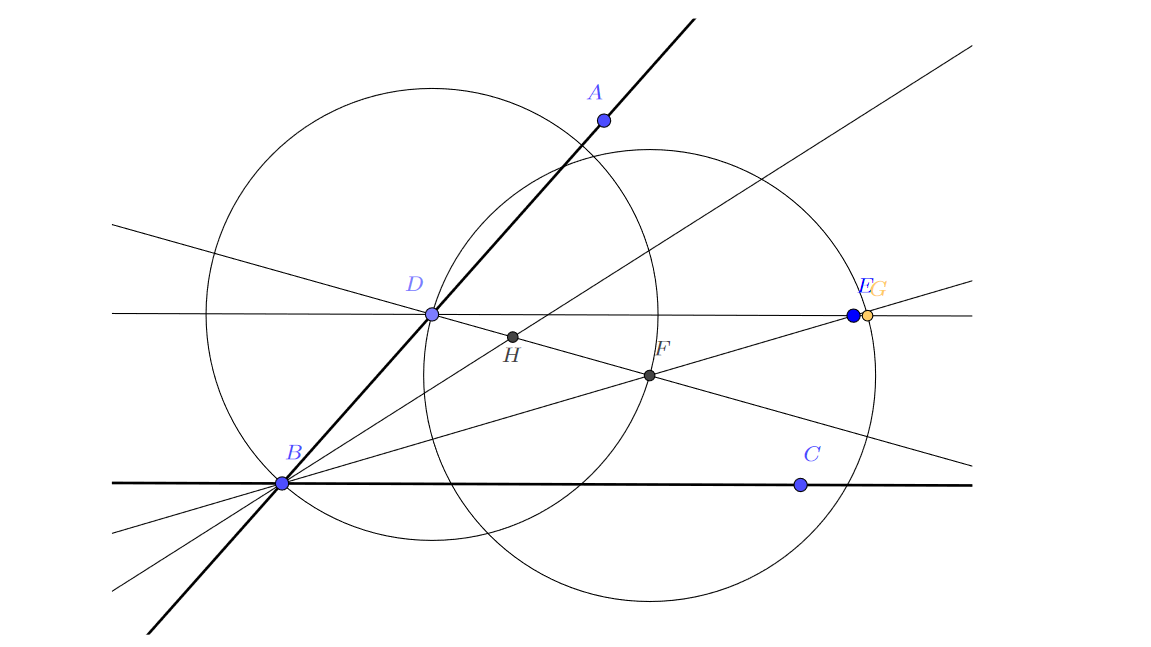
\includegraphics[width = \textwidth]{trisectangle.png}
\end{center}


\begin{enumerate}
   

  \item Prove that $\triangle DFE$ and $\triangle BDF$ are isosceles.\\
  \textbf{Answer:} Consider that by construction $C_D(B) = C_D(F)$. Therefore it must be the case that $BD = DF$ and therefore $\triangle BDF$
  is isosceles. Furthermore by construction we know that $C_F(D) = C_F(G)$ which gives us that $DF = FG$. Note that later on we "move point $E$ over point $G$"
  so by construction we get that $FG = FE$. Therefore $DF = FE$ and $\triangle DFE$ is isosceles. 
  \vspace{.5in}
  \item Prove that $\angle DEB = \angle EBC$.\\
  \textbf{Answer:} By construction we know that $DE || BC$. With $BE$ as a transversal we get that  $\angle DEB = \angle EBC$ by alternate interior angles.
  \vspace{.5in}



  \item Prove that $\angle DBF = \angle DFB = 2\angle DEB = 2\angle EBC$. \\
  \textbf{Answer:} The first equality comes from noting that $\triangle BDF$ is isosceles and therefore through pons asinorum we know that $\angle DBF = \angle DFB$.
  To get the middle equality, first consider the sum of the angles of $\triangle BDE$,
  \begin{equation*}
    \angle DBF + \angle BDF + \angle FDE + \angle DEB = 180
  \end{equation*}
  Note summing the angles of $\triangle BDF$ we get that, 
  \begin{equation*}
    \angle BDF  = 180 - 2\angle DBF.
  \end{equation*} 
  Since $\triangle DFE$ is isosceles we know that by pons asinorum that $\angle FDE  = \angle DEB$. Thus by substitution we know that the sum of the angles 
  for $\triangle BDE$,
  \begin{align*}
    \angle DBF + \angle BDF + \angle FDE + \angle DEB &= 180,\\
    \angle DBF + 180 - 2\angle DBF + 2\angle DEB &= 180,\\
    -\angle DBF + 2\angle DEB &= 0,\\
    2\angle DEB &= \angle DBF.
  \end{align*}
  Finally we get that last equality by substitution of the previous claim $\angle DEB = \angle EBC$.
  \vspace{.5in}
  
  
  
  \item Show that $\angle EBC = \frac{1}{3}(\angle EBC + \angle DBF) = \frac{1}{3}\angle CBD$.\\
  
  \textbf{Answer:} Consider $\frac{1}{3}(\angle EBC + \angle DBF)$. By the last claim we know that, $\angle DBF = 2\angle EBC$, 
  therefore by substitution we get that, 
  \begin{equation*}
    \angle EBC = \frac{1}{3}(\angle EBC + \angle DBF).
  \end{equation*}
  By addition we know that $\angle EBC + \angle DBF = \angle CBD$. Thus by substitution we get that,
  \begin{equation*}
    \frac{1}{3}(\angle EBC + \angle DBF) = \frac{1}{3}\angle CBD.
  \end{equation*}
  \vspace{.5in}

\end{enumerate}
\vspace{.5in}








\textbf{Section 4.2}
\begin{enumerate}
\item Proposition 6. If two angles of a triangle are congruent with one another, then the sides opposite those angles will also be 
congruent.\\
 
\textbf{Answer:} Suppose for the sake of contradiction that for $\triangle ACB$ we know that $\angle ABC = \angle ACB$, let 
$AB \neq AC$. Since $AC \neq BC$ assume $AB > AC$. There exists some point $D$ on $AB$ where $DB = AC$. Consider $\triangle ACB$ and 
$\triangle DBC$ and note that the share a base $BC$ and also have $DB = AC$ therefore by SS, $\triangle ACB \cong \triangle DBC$, thus a contradiction. 
\vspace{.5in}

\setcounter{enumi}{6}
\item If two opposite sides of a quadrilateral are equal and parallel, then the other two sides are also equal and parallel.\\
\begin{center}
  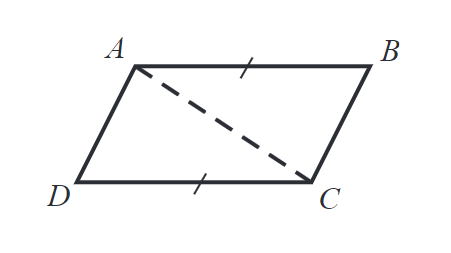
\includegraphics[width = .50\textwidth]{parallel.png}
\end{center}
\textbf{Answer:} Consider the parallelogram $ABCD$ with $AB = DC$ and that $AB || DC$. Consider the transversal $AC$. By alternate interior angles
we know that $\angle BAC = \angle DCA$. Therefore $\triangle ABC \cong \triangle ADC$ by SAS. Therefore by congruency we know that $AD = BC$. Now consider the sum of
the angles for $\triangle ABC$,
\begin{equation*}
  \angle BAC + \angle ACB + \angle CBA = 180. 
\end{equation*} 
By alternate interior angles we know that $\angle ACB = \angle DAC$, thus by substitution, 
\begin{equation*}
  \angle BAC + \angle DAC + \angle CBA = 180.
\end{equation*}
By Euclid's parallel postulate we know that $AD || BC$. 
\vspace{.5in}


\setcounter{enumi}{11}


\item The Greeks constructed a line segment of length $\sqrt{n}$, where $n$ is a positive integer, as 
follows. First write $n$ as $n \dot 1;$ then make $AB = n$ and $BC = 1$. Draw a semicircle on $AC$ diameter. Erect $BD$ 
perpendicular to $AC$ to $B$, meeting the semicircle at the point $D$. By similar triangles, prove that the length of $BD$ equals $\sqrt{n}$.\\
\begin{center}
  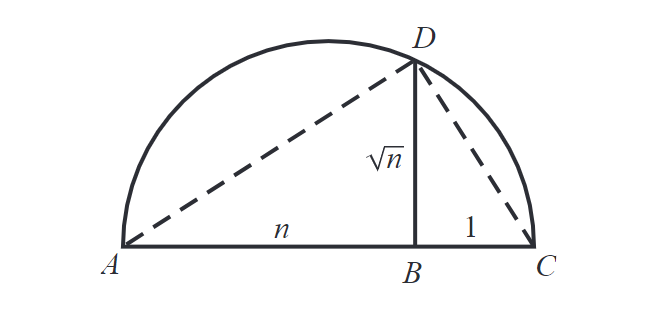
\includegraphics[width = .50\textwidth]{rootn.png}
\end{center}  

\textbf{Answer:} First note that by the Carpenter's Lemma we know that $\triangle CDA$ is a right triangle, where $\angle CDA = 90$. 
Now note that $\angle BAD = \angle CAD$ and therefore $\triangle CDA \sim \triangle DBA$ by AA similarity. Also note that $\angle DCA = \angle BCD$
and therefore we know that $\triangle CDA \sim \triangle CBD$ by AA similarity. Applying the Pythagorean Theorem to all three right triangles we know that, 
\begin{equation*}
  1^2 + DB^2 = DC^2,
\end{equation*} 
\begin{equation*}
  n^2 + DB^2 = AD^2,
\end{equation*} 
\begin{equation*}
  DC^2 + AD^2 = (n+1)^2.
\end{equation*} 
Substituting into the last equation we get that,
\begin{align*}
  1^2 + DB^2 + n^2 + DB^2 &= (n+1)^2,\\
  n^2 + 2DB^2 + 1 &= n^2 + 2n + 1,\\
  DB^2&= n.
\end{align*}
Thus $DB =\sqrt{n}$


\vspace{.5in}





\setcounter{enumi}{10}
\item The following is a few constructions of Pappus's Theorem using GeoGebra. To use my construction I had to 
move the bottom parallelogram around do that the circle intersects with the triangle and the ray $SA$ intersects $H$. I had a hard time trying to set 
the height of the bottom parallelogram so the areas didn't line up perfectly. 
\textbf{Answer:} 
\begin{center}
  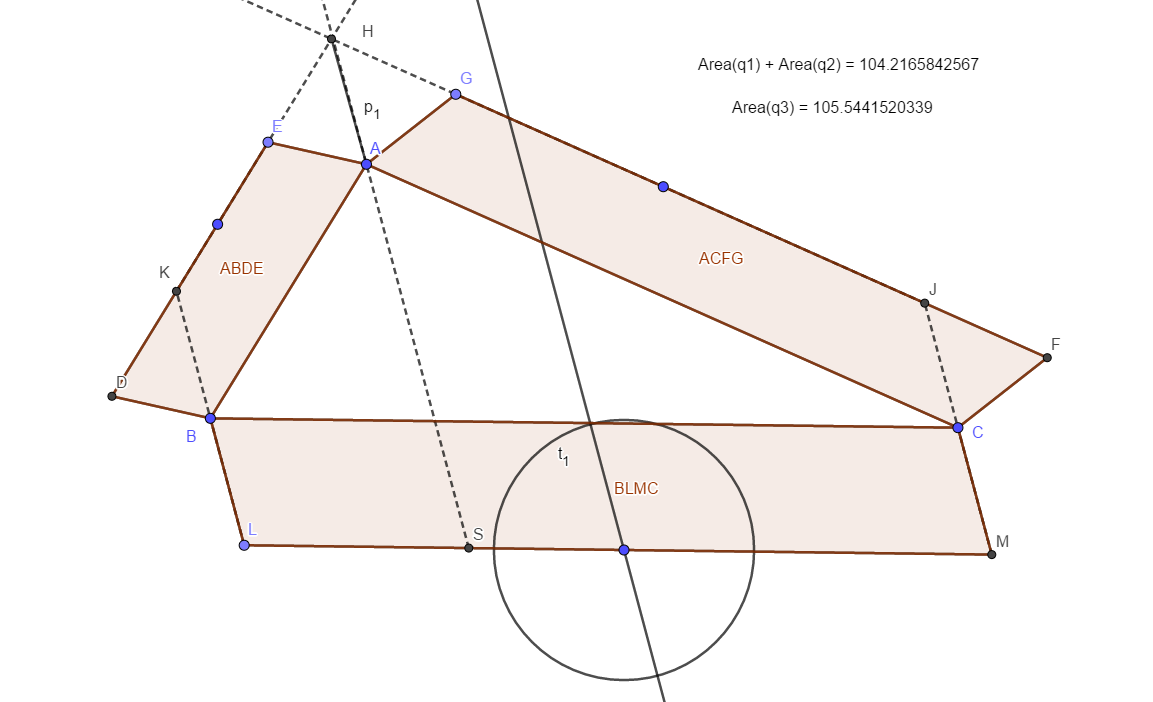
\includegraphics[width = .90\textwidth]{geogebraconstruction.png}
\end{center}  
\begin{center}
  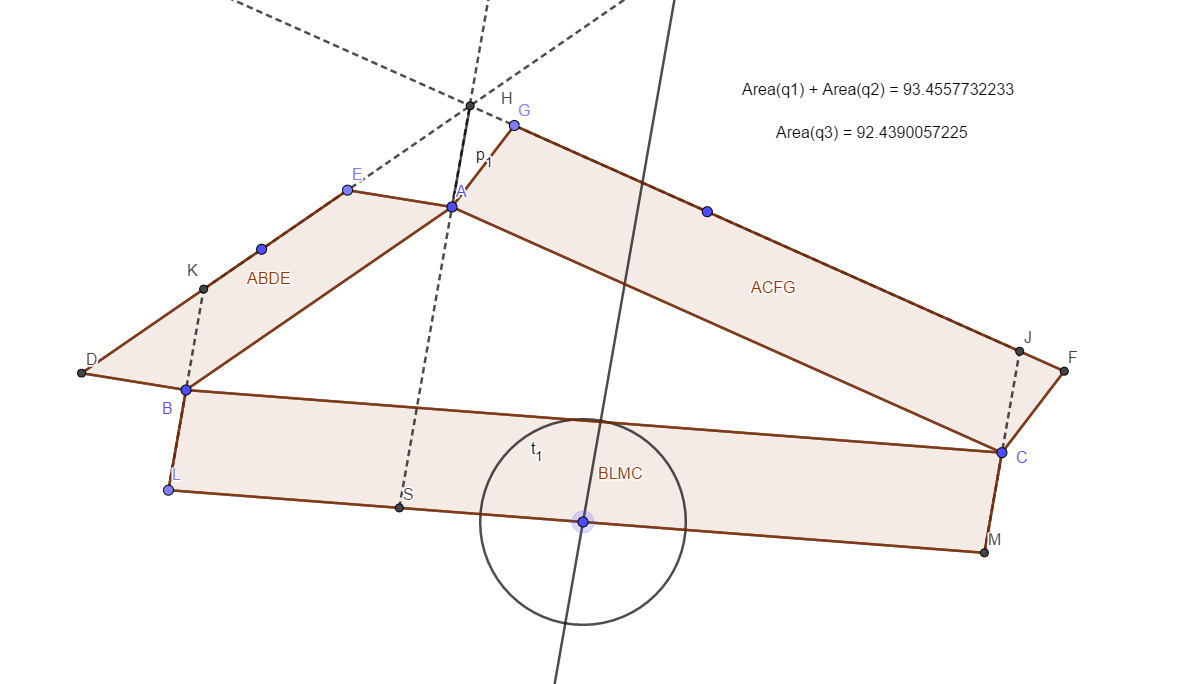
\includegraphics[width = .90\textwidth]{geogebraconstruction1.png}
\end{center}  
\begin{center}
  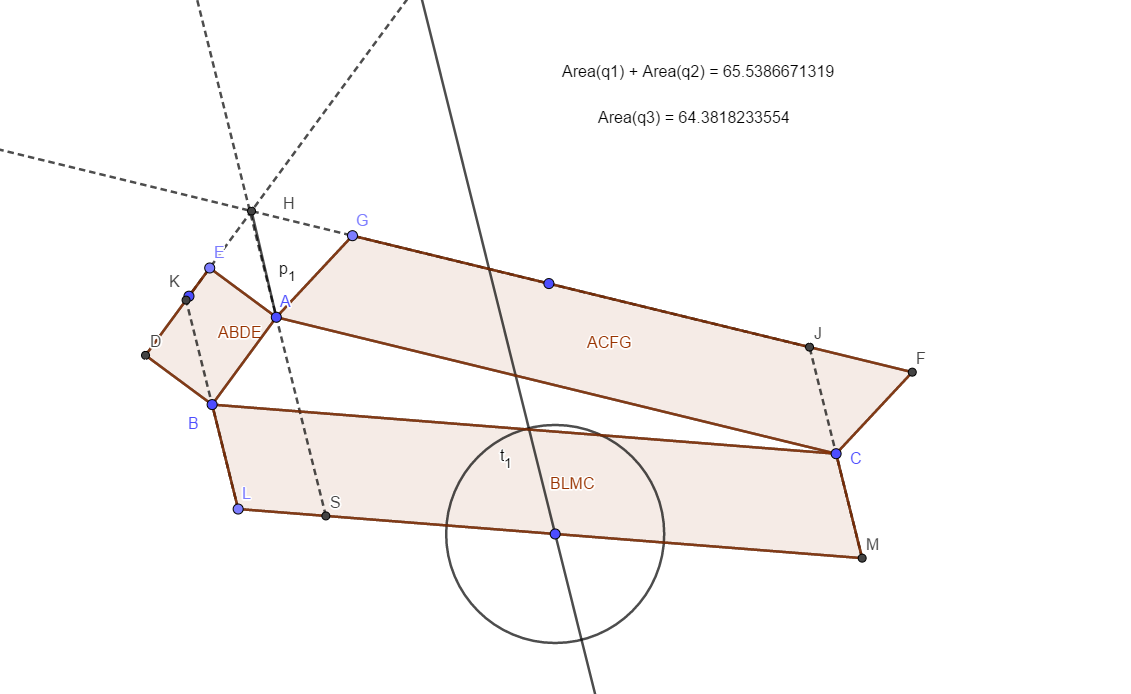
\includegraphics[width = .90\textwidth]{geogebraconstruction2.png}
\end{center}  






\vspace{.5in}

\end{enumerate}
\vspace{.5in}



\textbf{Reflection:}
\begin{enumerate}
\item I had a lot of trouble with the GeoGebra construction. The big issue was getting the height of the bottom parallelogram set to the length of segment $HA$. 
What I ended up doing was just trying to line it up manually similarly to the trisect the angle construction. It kind of worked but I think if I did it again I could get the areas to be exact. 
\item It took me a long time to see the algebra for the $\sqrt{n}$ problem. It really helped me just to list out all the relationships I knew, pythagorean theorems and side ratios for similar triangles. 
\end{enumerate}





\end{document}